\documentclass{article}\usepackage[]{graphicx}\usepackage[]{color}
%% maxwidth is the original width if it is less than linewidth
%% otherwise use linewidth (to make sure the graphics do not exceed the margin)
\makeatletter
\def\maxwidth{ %
  \ifdim\Gin@nat@width>\linewidth
    \linewidth
  \else
    \Gin@nat@width
  \fi
}
\makeatother

\definecolor{fgcolor}{rgb}{0.345, 0.345, 0.345}
\newcommand{\hlnum}[1]{\textcolor[rgb]{0.686,0.059,0.569}{#1}}%
\newcommand{\hlstr}[1]{\textcolor[rgb]{0.192,0.494,0.8}{#1}}%
\newcommand{\hlcom}[1]{\textcolor[rgb]{0.678,0.584,0.686}{\textit{#1}}}%
\newcommand{\hlopt}[1]{\textcolor[rgb]{0,0,0}{#1}}%
\newcommand{\hlstd}[1]{\textcolor[rgb]{0.345,0.345,0.345}{#1}}%
\newcommand{\hlkwa}[1]{\textcolor[rgb]{0.161,0.373,0.58}{\textbf{#1}}}%
\newcommand{\hlkwb}[1]{\textcolor[rgb]{0.69,0.353,0.396}{#1}}%
\newcommand{\hlkwc}[1]{\textcolor[rgb]{0.333,0.667,0.333}{#1}}%
\newcommand{\hlkwd}[1]{\textcolor[rgb]{0.737,0.353,0.396}{\textbf{#1}}}%
\let\hlipl\hlkwb

\usepackage{framed}
\makeatletter
\newenvironment{kframe}{%
 \def\at@end@of@kframe{}%
 \ifinner\ifhmode%
  \def\at@end@of@kframe{\end{minipage}}%
  \begin{minipage}{\columnwidth}%
 \fi\fi%
 \def\FrameCommand##1{\hskip\@totalleftmargin \hskip-\fboxsep
 \colorbox{shadecolor}{##1}\hskip-\fboxsep
     % There is no \\@totalrightmargin, so:
     \hskip-\linewidth \hskip-\@totalleftmargin \hskip\columnwidth}%
 \MakeFramed {\advance\hsize-\width
   \@totalleftmargin\z@ \linewidth\hsize
   \@setminipage}}%
 {\par\unskip\endMakeFramed%
 \at@end@of@kframe}
\makeatother

\definecolor{shadecolor}{rgb}{.97, .97, .97}
\definecolor{messagecolor}{rgb}{0, 0, 0}
\definecolor{warningcolor}{rgb}{1, 0, 1}
\definecolor{errorcolor}{rgb}{1, 0, 0}
\newenvironment{knitrout}{}{} % an empty environment to be redefined in TeX

\usepackage{alltt}

\usepackage{amsmath, amssymb}
\usepackage{graphicx}
\usepackage{hyperref}
\IfFileExists{upquote.sty}{\usepackage{upquote}}{}
\begin{document}
\SweaveOpts{concordance=TRUE}

\title{Pol Sci 630: Problem Set 4 Solution - Regression Model Estimation}

\author{Prepared by: Anh Le (\href{mailto:anh.le@duke.edu}{anh.le@duke.edu})}

\date{Due Date: Wed, September 28, 2015 (Beginning of Class)}

\maketitle

\section{Subset data frame}

\subsection{Download data}

Download the following data from \verb`WDI` and clean it as follows. Briefly comment on what each command does.

\begin{knitrout}
\definecolor{shadecolor}{rgb}{0.969, 0.969, 0.969}\color{fgcolor}\begin{kframe}
\begin{alltt}
\hlkwd{library}\hlstd{(WDI)}
\end{alltt}


{\ttfamily\noindent\itshape\color{messagecolor}{\#\# Loading required package: RJSONIO}}\begin{alltt}
\hlstd{d_wdi} \hlkwb{<-} \hlkwd{WDI}\hlstd{(}\hlkwc{indicator} \hlstd{=} \hlkwd{c}\hlstd{(}\hlstr{"NY.GDP.PCAP.CD"}\hlstd{,} \hlstr{"SP.DYN.IMRT.IN"}\hlstd{,} \hlstr{"SH.MED.PHYS.ZS"}\hlstd{),}
             \hlkwc{start} \hlstd{=} \hlnum{2005}\hlstd{,} \hlkwc{end} \hlstd{=} \hlnum{2010}\hlstd{,} \hlkwc{extra} \hlstd{=} \hlnum{TRUE}\hlstd{)}
\hlstd{d_wdi} \hlkwb{<-} \hlstd{d_wdi[d_wdi}\hlopt{$}\hlstd{region} \hlopt{!=} \hlstr{"Aggregates"}\hlstd{,}
       \hlkwd{c}\hlstd{(}\hlstr{"country"}\hlstd{,} \hlstr{"year"}\hlstd{,} \hlstr{"NY.GDP.PCAP.CD"}\hlstd{,} \hlstr{"SP.DYN.IMRT.IN"}\hlstd{,} \hlstr{"SH.MED.PHYS.ZS"}\hlstd{)]}
\hlkwd{colnames}\hlstd{(d_wdi)[}\hlnum{3}\hlopt{:}\hlnum{5}\hlstd{]} \hlkwb{<-} \hlkwd{c}\hlstd{(}\hlstr{'gdppc'}\hlstd{,} \hlstr{'infant_mortality'}\hlstd{,} \hlstr{'number_of_physician'}\hlstd{)}
\hlstd{d_wdi} \hlkwb{<-} \hlkwd{na.omit}\hlstd{(d_wdi)}
\end{alltt}
\end{kframe}
\end{knitrout}

\verb`infant_mortality`: number of mortality per 1000 live births

\verb`number_of_physician`: number of physician per 1000 people

\subsection{Subsetting}

Use subsetting techniques to do the following:

\begin{enumerate}
\item Show the GDP per capita of Brazil across years
\item Show the country-years where infant mortality $>$ 100 per 1000 live birth
\item Show the country-years where GDP per capita is above average
\item Show the country-years where GDP per capita is above average, but number of physician is below average
\end{enumerate}

\textbf{Solution}

\begin{knitrout}
\definecolor{shadecolor}{rgb}{0.969, 0.969, 0.969}\color{fgcolor}\begin{kframe}
\begin{alltt}
\hlkwd{library}\hlstd{(WDI)}

\hlcom{# Download data from WDI, specifying the indicators and start / end year}
\hlstd{d_wdi} \hlkwb{<-} \hlkwd{WDI}\hlstd{(}\hlkwc{indicator} \hlstd{=} \hlkwd{c}\hlstd{(}\hlstr{"NY.GDP.PCAP.CD"}\hlstd{,} \hlstr{"SP.DYN.IMRT.IN"}\hlstd{,} \hlstr{"SH.MED.PHYS.ZS"}\hlstd{),}
             \hlkwc{start} \hlstd{=} \hlnum{2008}\hlstd{,} \hlkwc{end} \hlstd{=} \hlnum{2010}\hlstd{,} \hlkwc{extra} \hlstd{=} \hlnum{TRUE}\hlstd{)}

\hlcom{# Remove aggregates rows, selecting wanted columns by name}
\hlstd{d_wdi} \hlkwb{<-} \hlstd{d_wdi[d_wdi}\hlopt{$}\hlstd{region} \hlopt{!=} \hlstr{"Aggregates"}\hlstd{,}
       \hlkwd{c}\hlstd{(}\hlstr{"country"}\hlstd{,} \hlstr{"year"}\hlstd{,} \hlstr{"NY.GDP.PCAP.CD"}\hlstd{,} \hlstr{"SP.DYN.IMRT.IN"}\hlstd{,} \hlstr{"SH.MED.PHYS.ZS"}\hlstd{)]}

\hlcom{# Rename some of the columns}
\hlkwd{colnames}\hlstd{(d_wdi)[}\hlnum{3}\hlopt{:}\hlnum{5}\hlstd{]} \hlkwb{<-} \hlkwd{c}\hlstd{(}\hlstr{'gdppc'}\hlstd{,} \hlstr{'infant_mortality'}\hlstd{,} \hlstr{'number_of_physician'}\hlstd{)}

\hlcom{# Remove all rows that have missing data}
\hlstd{d_wdi} \hlkwb{<-} \hlkwd{na.omit}\hlstd{(d_wdi)}
\end{alltt}
\end{kframe}
\end{knitrout}

\begin{knitrout}
\definecolor{shadecolor}{rgb}{0.969, 0.969, 0.969}\color{fgcolor}\begin{kframe}
\begin{alltt}
\hlcom{# 1. Show the GDP per capita of Brazil across years}
\hlstd{d_wdi[d_wdi}\hlopt{$}\hlstd{country} \hlopt{==} \hlstr{"Brazil"}\hlstd{,} \hlkwd{c}\hlstd{(}\hlstr{"country"}\hlstd{,} \hlstr{"year"}\hlstd{,} \hlstr{"gdppc"}\hlstd{)]}
\end{alltt}
\begin{verbatim}
##    country year     gdppc
## 94  Brazil 2008  8706.819
## 95  Brazil 2009  8474.881
## 96  Brazil 2010 11121.421
\end{verbatim}
\begin{alltt}
\hlcom{# 2. Show the country-years where infant mortality > 100 per 1000 live birth}
\hlstd{d_wdi[d_wdi}\hlopt{$}\hlstd{infant_mortality} \hlopt{>} \hlnum{100}\hlstd{,} \hlkwd{c}\hlstd{(}\hlstr{"country"}\hlstd{,} \hlstr{"year"}\hlstd{,} \hlstr{"infant_mortality"}\hlstd{)]}
\end{alltt}
\begin{verbatim}
##                      country year infant_mortality
## 34                    Angola 2009            112.2
## 119 Central African Republic 2008            105.5
## 120 Central African Republic 2009            103.6
## 568             Sierra Leone 2010            107.0
## 570             Sierra Leone 2008            116.2
\end{verbatim}
\begin{alltt}
\hlcom{# 3. Show the country-years where GDP per capita is above average}
\hlstd{d_wdi[d_wdi}\hlopt{$}\hlstd{gdppc} \hlopt{>} \hlkwd{mean}\hlstd{(d_wdi}\hlopt{$}\hlstd{gdppc),} \hlkwd{c}\hlstd{(}\hlstr{"country"}\hlstd{,} \hlstr{"year"}\hlstd{,} \hlstr{"gdppc"}\hlstd{)]}
\end{alltt}
\begin{verbatim}
##                  country year     gdppc
## 16               Andorra 2009  42701.45
## 17               Andorra 2010  39639.39
## 19  United Arab Emirates 2009  32905.05
## 20  United Arab Emirates 2008  45720.02
## 21  United Arab Emirates 2010  34341.91
## 44               Austria 2010  46659.84
## 46             Australia 2009  42715.13
## 47             Australia 2010  51845.65
## 63              Barbados 2010  15901.43
## 67               Belgium 2010  44382.88
## 68               Belgium 2008  48424.59
## 76               Bahrain 2010  20386.02
## 77               Bahrain 2008  23043.03
## 78               Bahrain 2009  19166.71
## 88     Brunei Darussalam 2009  27726.48
## 89     Brunei Darussalam 2010  31453.22
## 90     Brunei Darussalam 2008  37798.39
## 99          Bahamas, The 2008  23657.37
## 112               Canada 2008  46596.34
## 114               Canada 2010  47445.76
## 124          Switzerland 2010  74277.12
## 154               Cyprus 2008  34950.35
## 155               Cyprus 2009  31673.46
## 156               Cyprus 2010  30438.90
## 157       Czech Republic 2010  19763.96
## 158       Czech Republic 2008  22649.38
## 160              Germany 2010  41788.04
## 162              Germany 2008  45699.20
## 166              Denmark 2010  57647.67
## 167              Denmark 2009  57895.50
## 168              Denmark 2008  64181.99
## 181              Estonia 2008  18094.55
## 183              Estonia 2010  14641.40
## 190                Spain 2009  32333.47
## 191                Spain 2010  30737.83
## 192                Spain 2008  35578.74
## 202              Finland 2010  46205.17
## 203              Finland 2008  53401.31
## 204              Finland 2009  47107.16
## 214               France 2008  45413.07
## 215               France 2010  40705.77
## 222       United Kingdom 2010  38292.87
## 247               Greece 2010  26919.36
## 248               Greece 2008  31997.28
## 268              Croatia 2008  15893.86
## 275              Hungary 2008  15649.72
## 280              Ireland 2008  61189.73
## 282              Ireland 2010  48260.67
## 283               Israel 2010  30736.36
## 298              Iceland 2010  41620.07
## 299              Iceland 2008  55229.61
## 300              Iceland 2009  40362.04
## 301                Italy 2009  36976.85
## 302                Italy 2010  35851.51
## 303                Italy 2008  40640.18
## 313                Japan 2010  42935.25
## 315                Japan 2008  37865.62
## 337          Korea, Rep. 2008  20474.89
## 338          Korea, Rep. 2010  22151.21
## 339          Korea, Rep. 2009  18338.71
## 340               Kuwait 2009  36754.95
## 341               Kuwait 2008  54484.30
## 342               Kuwait 2010  37725.14
## 371            Lithuania 2008  14961.57
## 373           Luxembourg 2010 103267.28
## 377               Latvia 2008  16323.77
## 381                Libya 2008  14231.60
## 425                Malta 2010  19694.08
## 426                Malta 2009  19636.01
## 460          Netherlands 2010  50341.25
## 462          Netherlands 2008  56928.82
## 463               Norway 2010  87646.27
## 464               Norway 2009  80017.78
## 465               Norway 2008  96880.51
## 472          New Zealand 2009  28200.94
## 473          New Zealand 2008  31287.61
## 474          New Zealand 2010  33692.17
## 478                 Oman 2009  17518.83
## 479                 Oman 2010  19920.65
## 480                 Oman 2008  22963.38
## 501               Poland 2008  13906.22
## 508             Portugal 2008  24815.61
## 509             Portugal 2010  22540.00
## 510             Portugal 2009  23063.97
## 517                Qatar 2008  82990.07
## 518                Qatar 2010  70870.23
## 519                Qatar 2009  61463.90
## 544         Saudi Arabia 2008  19436.86
## 545         Saudi Arabia 2009  15655.08
## 546         Saudi Arabia 2010  18753.98
## 556               Sweden 2008  55746.84
## 557               Sweden 2010  52076.43
## 558               Sweden 2009  46207.06
## 559            Singapore 2009  38577.56
## 560            Singapore 2010  46569.68
## 561            Singapore 2008  39721.05
## 562             Slovenia 2010  23438.85
## 564             Slovenia 2008  27501.82
## 565      Slovak Republic 2009  16460.22
## 566      Slovak Republic 2010  16554.88
## 650  Trinidad and Tobago 2010  15840.44
## 664        United States 2010  48374.09
## 665        United States 2009  47001.56
## 666        United States 2008  48401.43
\end{verbatim}
\begin{alltt}
\hlcom{# 4. Show the country-years where GDP per capita is above average,}
\hlcom{# but number of physician is below average}
\hlstd{d_wdi[d_wdi}\hlopt{$}\hlstd{gdppc} \hlopt{>} \hlkwd{mean}\hlstd{(d_wdi}\hlopt{$}\hlstd{gdppc)} \hlopt{&}
        \hlstd{d_wdi}\hlopt{$}\hlstd{number_of_physician} \hlopt{<} \hlkwd{mean}\hlstd{(d_wdi}\hlopt{$}\hlstd{number_of_physician),}
      \hlkwd{c}\hlstd{(}\hlstr{"country"}\hlstd{,} \hlstr{"year"}\hlstd{,} \hlstr{"gdppc"}\hlstd{)]}
\end{alltt}
\begin{verbatim}
##                 country year    gdppc
## 76              Bahrain 2010 20386.02
## 77              Bahrain 2008 23043.03
## 78              Bahrain 2009 19166.71
## 88    Brunei Darussalam 2009 27726.48
## 89    Brunei Darussalam 2010 31453.22
## 90    Brunei Darussalam 2008 37798.39
## 341              Kuwait 2008 54484.30
## 561           Singapore 2008 39721.05
## 650 Trinidad and Tobago 2010 15840.44
\end{verbatim}
\end{kframe}
\end{knitrout}

\section{Build linear model}

\subsection{Download}

Download 2 variables of interest and build a linear model of their relationship using \verb`lm()`. Show the \verb`summary()` of results.

\subsection{Calculate the regression coefficients WITHOUT using `lm`}

Use the mathematical formula of the regression coefficients you saw in class and implement it in R. Is this result the same as the result output by `lm`?

\subsection{Model output}

Show the result with \verb`stargazer`, customizing:
\begin{itemize}
\item The labels of the independent variables (i.e. the covariate)
\item The label of the dependent variable
\item Make the model name (i.e. OLS) show up
\end{itemize}

Hint: The options to do those things are in \verb`help(stargazer)`. I have worded the task in a way that should help you find the relevant options.

\textbf{Solution}

Build the linear model

\begin{knitrout}
\definecolor{shadecolor}{rgb}{0.969, 0.969, 0.969}\color{fgcolor}\begin{kframe}
\begin{alltt}
\hlstd{m1} \hlkwb{<-} \hlkwd{lm}\hlstd{(infant_mortality} \hlopt{~} \hlstd{gdppc,} \hlkwc{data} \hlstd{= d_wdi)}
\hlkwd{summary}\hlstd{(m1)}
\end{alltt}
\begin{verbatim}
## 
## Call:
## lm(formula = infant_mortality ~ gdppc, data = d_wdi)
## 
## Residuals:
##     Min      1Q  Median      3Q     Max 
## -27.697 -16.248  -6.166  11.606  80.199 
## 
## Coefficients:
##               Estimate Std. Error t value Pr(>|t|)    
## (Intercept)  3.633e+01  1.384e+00   26.25   <2e-16 ***
## gdppc       -7.307e-04  5.933e-05  -12.32   <2e-16 ***
## ---
## Signif. codes:  0 '***' 0.001 '**' 0.01 '*' 0.05 '.' 0.1 ' ' 1
## 
## Residual standard error: 20.9 on 350 degrees of freedom
## Multiple R-squared:  0.3024,	Adjusted R-squared:  0.3004 
## F-statistic: 151.7 on 1 and 350 DF,  p-value: < 2.2e-16
\end{verbatim}
\end{kframe}
\end{knitrout}

Calculate the regression coef by hand, using covariance and variance:

\begin{knitrout}
\definecolor{shadecolor}{rgb}{0.969, 0.969, 0.969}\color{fgcolor}\begin{kframe}
\begin{alltt}
\hlkwd{cov}\hlstd{(d_wdi}\hlopt{$}\hlstd{infant_mortality, d_wdi}\hlopt{$}\hlstd{gdppc)} \hlopt{/} \hlkwd{var}\hlstd{(d_wdi}\hlopt{$}\hlstd{gdppc)}
\end{alltt}
\begin{verbatim}
## [1] -0.00073073
\end{verbatim}
\end{kframe}
\end{knitrout}

or fully by hand (the result will be slightly different because R's `cov` and `var` divided by `n - 1` while `mean` divides by `n`) (read more at \url{http://nebula.deanza.edu/~bloom/math10/m10divideby_nminus1.pdf}):

\begin{knitrout}
\definecolor{shadecolor}{rgb}{0.969, 0.969, 0.969}\color{fgcolor}\begin{kframe}
\begin{alltt}
\hlkwd{mean}\hlstd{((d_wdi}\hlopt{$}\hlstd{infant_mortality} \hlopt{-} \hlkwd{mean}\hlstd{(d_wdi}\hlopt{$}\hlstd{infant_mortality))} \hlopt{*}
       \hlstd{d_wdi}\hlopt{$}\hlstd{gdppc} \hlopt{-} \hlkwd{mean}\hlstd{(d_wdi}\hlopt{$}\hlstd{gdppc))} \hlopt{/}
  \hlkwd{mean}\hlstd{((d_wdi}\hlopt{$}\hlstd{gdppc} \hlopt{-} \hlkwd{mean}\hlstd{(d_wdi}\hlopt{$}\hlstd{gdppc))}\hlopt{**}\hlnum{2}\hlstd{)}
\end{alltt}
\begin{verbatim}
## [1] -0.0007699624
\end{verbatim}
\end{kframe}
\end{knitrout}



\begin{kframe}
\begin{alltt}
\hlkwd{library}\hlstd{(stargazer)}
\end{alltt}


{\ttfamily\noindent\itshape\color{messagecolor}{\#\# \\\#\# Please cite as:}}

{\ttfamily\noindent\itshape\color{messagecolor}{\#\#\ \ Hlavac, Marek (2015). stargazer: Well-Formatted Regression and Summary Statistics Tables.}}

{\ttfamily\noindent\itshape\color{messagecolor}{\#\#\ \ R package version 5.2. http://CRAN.R-project.org/package=stargazer}}\begin{alltt}
\hlkwd{stargazer}\hlstd{(m1,}
          \hlkwc{covariate.labels} \hlstd{=} \hlkwd{c}\hlstd{(}\hlstr{"GDP per capita"}\hlstd{),}
          \hlkwc{dep.var.labels} \hlstd{=} \hlkwd{c}\hlstd{(}\hlstr{"Infant Mortality (per 1000 births)"}\hlstd{),}
          \hlkwc{model.names} \hlstd{=} \hlnum{TRUE}\hlstd{)}
\end{alltt}
\end{kframe}
% Table created by stargazer v.5.2 by Marek Hlavac, Harvard University. E-mail: hlavac at fas.harvard.edu
% Date and time: Fri, Sep 23, 2016 - 02:15:33 PM
\begin{table}[!htbp] \centering 
  \caption{} 
  \label{} 
\begin{tabular}{@{\extracolsep{5pt}}lc} 
\\[-1.8ex]\hline 
\hline \\[-1.8ex] 
 & \multicolumn{1}{c}{\textit{Dependent variable:}} \\ 
\cline{2-2} 
\\[-1.8ex] & Infant Mortality (per 1000 births) \\ 
\\[-1.8ex] & \textit{OLS} \\ 
\hline \\[-1.8ex] 
 GDP per capita & $-$0.001$^{***}$ \\ 
  & (0.0001) \\ 
  & \\ 
 Constant & 36.332$^{***}$ \\ 
  & (1.384) \\ 
  & \\ 
\hline \\[-1.8ex] 
Observations & 352 \\ 
R$^{2}$ & 0.302 \\ 
Adjusted R$^{2}$ & 0.300 \\ 
Residual Std. Error & 20.905 (df = 350) \\ 
F Statistic & 151.705$^{***}$ (df = 1; 350) \\ 
\hline 
\hline \\[-1.8ex] 
\textit{Note:}  & \multicolumn{1}{r}{$^{*}$p$<$0.1; $^{**}$p$<$0.05; $^{***}$p$<$0.01} \\ 
\end{tabular} 
\end{table} 


\section{Calculate sum of squares and RMSE}

\begin{enumerate}
\item Extract the residuals and predicted values (fitted values) from the model object (from the linear model built above)
\item Calculate three ``sum of squares'' (TSS, RegSS, RSS)
\item Calculate the root mean square error and compare with R. (In R and stargazer, RMSE is called ``Residual standard error''.)
\end{enumerate}

Note: the data you feed to \verb`lm()` may have missing data, so R has to modify the data a little before using it. To extract the data that are actually used by \verb`lm()`, use \verb`my_model$model`. Use this data to calculate $\bar y$ in the sum of squares.

\textbf{Solution}

\begin{knitrout}
\definecolor{shadecolor}{rgb}{0.969, 0.969, 0.969}\color{fgcolor}\begin{kframe}
\begin{alltt}
\hlstd{res} \hlkwb{<-} \hlstd{m1}\hlopt{$}\hlstd{residuals} \hlcom{# Residuals}
\hlstd{pred} \hlkwb{<-} \hlstd{m1}\hlopt{$}\hlstd{fitted.values} \hlcom{# Predicted values}
\hlstd{y} \hlkwb{<-} \hlstd{m1}\hlopt{$}\hlstd{model}\hlopt{$}\hlstd{infant_mortality} \hlcom{# Data of Y that is used by lm()}

\hlcom{# Calculate 3 sum of squares}
\hlstd{TSS} \hlkwb{<-} \hlkwd{sum}\hlstd{( (y} \hlopt{-} \hlkwd{mean}\hlstd{(y))} \hlopt{**} \hlnum{2}\hlstd{)}
\hlstd{RegSS} \hlkwb{<-} \hlkwd{sum}\hlstd{( (pred} \hlopt{-} \hlkwd{mean}\hlstd{(y))} \hlopt{**} \hlnum{2}\hlstd{)}
\hlstd{RSS} \hlkwb{<-} \hlkwd{sum}\hlstd{( res} \hlopt{**} \hlnum{2} \hlstd{)}

\hlcom{# Calculate root mean square error}
\hlstd{N} \hlkwb{<-} \hlkwd{nrow}\hlstd{(d_wdi)}
\hlstd{k} \hlkwb{<-} \hlnum{1} \hlcom{# We only have 1 predictor, which is log_gdppc}
\hlstd{rmse} \hlkwb{<-} \hlkwd{sqrt}\hlstd{(RSS} \hlopt{/} \hlstd{(N} \hlopt{-} \hlstd{k} \hlopt{-} \hlnum{1}\hlstd{))}
\end{alltt}
\end{kframe}
\end{knitrout}

The calculated root mean square error is 20.9048032, the same as reported by R in \verb`summary(m1)`.

\section{Explore why we have standard errors}

\begin{knitrout}
\definecolor{shadecolor}{rgb}{0.969, 0.969, 0.969}\color{fgcolor}\begin{kframe}
\begin{alltt}
\hlstd{x} \hlkwb{<-} \hlkwd{rnorm}\hlstd{(}\hlkwc{mean} \hlstd{=} \hlnum{5}\hlstd{,} \hlnum{100}\hlstd{)}
\hlstd{y} \hlkwb{<-} \hlnum{1} \hlopt{+} \hlnum{2} \hlopt{*} \hlstd{x} \hlopt{+} \hlkwd{rnorm}\hlstd{(}\hlnum{100}\hlstd{)}
\hlkwd{plot}\hlstd{(y, x)}

\hlstd{c_nsim} \hlkwb{<-} \hlnum{100}
\hlstd{model_data} \hlkwb{<-} \hlkwd{vector}\hlstd{(}\hlstr{"list"}\hlstd{,} \hlkwc{length} \hlstd{= c_nsim)}
\hlstd{model_results} \hlkwb{<-} \hlkwd{vector}\hlstd{(}\hlstr{"list"}\hlstd{,} \hlkwc{length} \hlstd{= c_nsim)}
\hlkwa{for} \hlstd{(i} \hlkwa{in} \hlnum{1}\hlopt{:}\hlstd{c_nsim) \{}
  \hlstd{sample_index} \hlkwb{<-} \hlkwd{sample}\hlstd{(}\hlnum{100}\hlstd{,} \hlnum{10}\hlstd{,} \hlkwc{replace} \hlstd{=} \hlnum{TRUE}\hlstd{)}
  \hlstd{sample_x} \hlkwb{<-} \hlstd{x[sample_index]}
  \hlstd{sample_y} \hlkwb{<-} \hlstd{y[sample_index]}
  \hlstd{model_data[[i]]} \hlkwb{<-} \hlkwd{list}\hlstd{(sample_x, sample_y)}
  \hlstd{model_results[[i]]} \hlkwb{<-} \hlkwd{lm}\hlstd{(sample_y} \hlopt{~} \hlstd{sample_x)}
\hlstd{\}}

\hlkwd{plot}\hlstd{(y, x)}
\end{alltt}
\end{kframe}
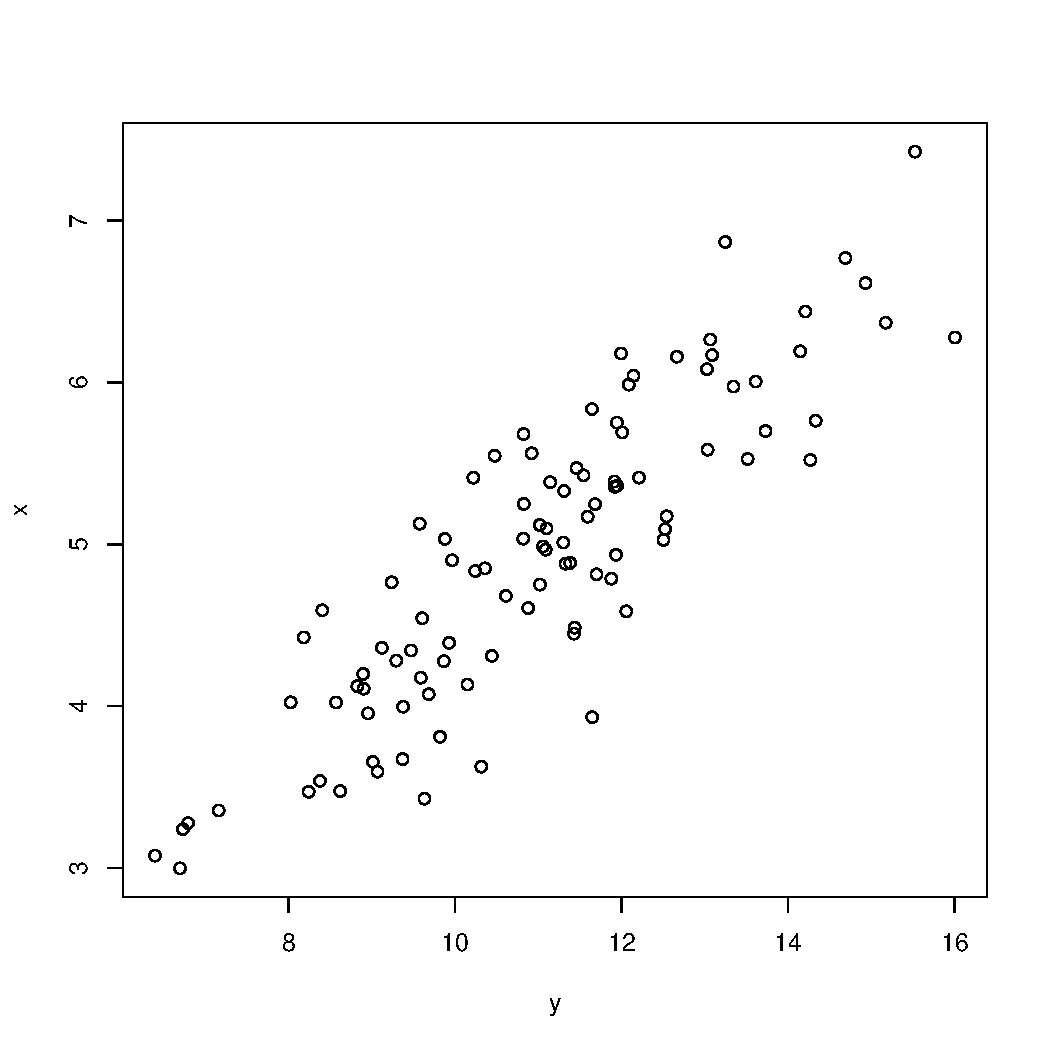
\includegraphics[width=\maxwidth]{figure/unnamed-chunk-9-1} 
\begin{kframe}\begin{alltt}
\hlkwa{for} \hlstd{(i} \hlkwa{in} \hlnum{1}\hlopt{:}\hlstd{c_nsim) \{}

\hlstd{\}}
\end{alltt}
\end{kframe}
\end{knitrout}


\end{document}
